% ============================================================================
%  informe_avance.tex - Informe de avance del proyecto Pong en FPGA
%  Electrónica Digital 1 - Universidad Nacional de Colombia, sede Bogotá
%  Juan David Ortiz Muñoz, David Eduardo Chivata Arias, Daniel Felipe Castro González
%  Compilar con: pdflatex informe_avance.tex (dos veces, por las referencias)
% ============================================================================
\documentclass[conference,a4paper]{IEEEtran}
\usepackage[utf8]{inputenc}
\usepackage[T1]{fontenc}
\usepackage[spanish,es-noshorthands,es-tabla]{babel}
\usepackage{lmodern}
\usepackage{graphicx}
\usepackage{booktabs}
\usepackage{tabularx}
\usepackage{array}
\usepackage{multirow}
\usepackage{xcolor}
\usepackage{url}
\usepackage[hidelinks]{hyperref}
\usepackage{newunicodechar}
\newunicodechar{Ω}{\ensuremath{\Omega}}
\newunicodechar{→}{\ensuremath{\rightarrow}}
\graphicspath{{../figuras/}{../../fases/F4_interfaz_visual/}}
\newcolumntype{Y}{>{\raggedright\arraybackslash}X}
\newcommand{\ok}{\textcolor{green!45!black}{\textbf{Cumplido}}}
\newcommand{\parcial}{\textcolor{orange!80!black}{\textbf{Parcial}}}
\newcommand{\pend}{\textcolor{red!70!black}{\textbf{Pendiente}}}

\begin{document}

% ============================================================================
% 1. Título
% ============================================================================
\title{Informe de avance: diseño e implementación de un videojuego Pong mediante electrónica digital con FPGA}

\author{\IEEEauthorblockN{Juan David Ortiz Muñoz, David Eduardo Chivata Arias y Daniel Felipe Castro González}
\IEEEauthorblockA{Departamento de Ingeniería Eléctrica y Electrónica\\
Universidad Nacional de Colombia, sede Bogotá\\
\{juaortizmu, dchivata, dcastrogon\}@unal.edu.co}}

\maketitle

\begin{abstract}
Presentamos el avance del proyecto Pong para dos jugadores en una FPGA Cyclone~IV~E EP4CE10E22C8N, con corte al 15 de noviembre de 2026. El juego ya funciona en protoboard: la FPGA calcula el movimiento de las paletas y la pelota, detecta impactos y goles, lleva el puntaje y dibuja el tablero en dos matrices LED de $8\times8$ en cascada (controlador compatible con MAX7219). El puntaje se muestra en dos displays de siete segmentos por medio de decodificadores CD4511BE, y todas las señales que salen de la FPGA a 3,3~V pasan por dos búferes SN74HCT245N alimentados a 5~V. En simulación pasan los 19 bancos de prueba y en hardware se jugó una partida completa hasta 9--6, con victoria, RESET y nueva partida. Frente al cronograma de la propuesta llevamos cerca del 88~\%. La diferencia más importante es que los controles inalámbricos se cambiaron por mandos cableados; quedan pendientes el arranque autónomo de la FPGA, la evidencia en video, la revisión eléctrica de las entradas y el diseño de las placas.
\end{abstract}

\begin{IEEEkeywords}
FPGA, Verilog, Pong, máquina de estados, MAX7219, CD4511BE, SN74HCT245N.
\end{IEEEkeywords}

% ============================================================================
% 2. Introducción
% ============================================================================
\section{Introducción}

En la propuesta planteamos diseñar, simular e implementar un Pong para dos jugadores usando solo lógica digital sobre una FPGA, sin microcontroladores~\cite{propuesta}. El juego nos sirve para juntar en un mismo sistema lo que se ve por separado en el curso: lógica combinacional para las colisiones, registros y contadores para las posiciones y el puntaje, y máquinas de estados para el control del juego y para la comunicación serial con la pantalla~\cite{mano,brown,tocci}.

Trabajamos por fases, siguiendo nuestra guía metodológica~\cite{guia}: especificación (F0), arquitectura (F1), diseño lógico formal con tablas de verdad, tablas de transición y ecuaciones (F2), descripción en Verilog y simulación (F3), prueba de la pantalla en la tarjeta (F4), controles (F5), integración del marcador y montaje (F6) e informe del funcionamiento en protoboard (F7). Cada fase dejó un documento y su evidencia, y todo está en el repositorio del proyecto~\cite{repo}.

Este informe resume la arquitectura que tenemos definida, el listado de sensores y actuadores, cuánto hemos avanzado frente al cronograma de la propuesta y qué nos falta para cerrar.

% ============================================================================
% 3. Arquitectura diseñada
% ============================================================================
\section{Arquitectura diseñada}

\subsection{Diagrama de bloques}

La Fig.~\ref{fig:sistema} muestra el sistema completo. La FPGA, con su reloj de 50~MHz, recibe las órdenes de los dos jugadores y de los tres pulsadores. Dentro de ella el diseño se divide en seis grupos: entradas (sincronización y antirrebote), control (FSM de seis estados y temporizadores), motor del juego (paletas, pelota y colisiones), puntaje, imagen (instantánea de posiciones, armado de filas y transmisor serial) y seguridad (reset de arranque y supervisor de fallos). Hacia afuera salen dos grupos de señales: tres líneas seriales para las matrices y ocho bits BCD para el marcador.

\begin{figure*}[!t]
  \centering
  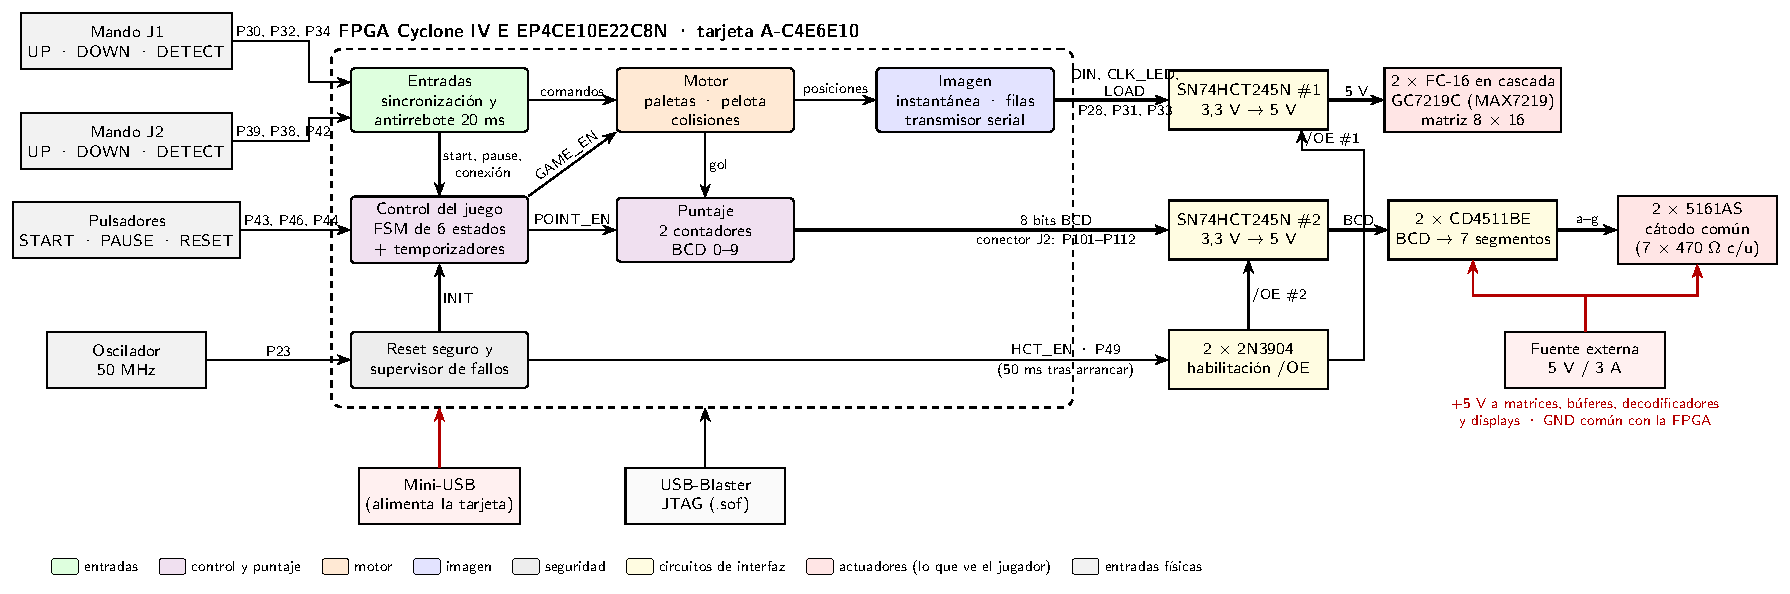
\includegraphics[width=\textwidth]{fig_sistema.pdf}
  \caption{Arquitectura del sistema montado en protoboard (versión F6). A la izquierda las entradas físicas con sus pines; en el centro los bloques que describimos en Verilog dentro de la FPGA; a la derecha los circuitos de interfaz y los actuadores.}
  \label{fig:sistema}
\end{figure*}

El núcleo en Verilog está compuesto por 15 módulos. Todos trabajan con el mismo reloj y avanzan con pulsos de habilitación: la pelota cada 200~ms y las paletas cada 250~ms. La FSM del juego tiene los estados ESPERA, JUEGO, PUNTO, PAUSA\_RF, FIN y PAUSA\_MANUAL, codificados en tres bits; los dos códigos que sobran se tratan como fallo y llevan al sistema a ESPERA. El transmisor tiene su propia FSM de 13 estados: primero manda las 14 instrucciones de configuración de los controladores y luego refresca las ocho filas, cada una como una trama de 32 bits (16 para cada matriz).

\subsection{Circuito}

La Fig.~\ref{fig:conexiones} es el circuito a nivel de pines, tal como quedó en el montaje de F6~\cite{f6}. Como los GPIO de la tarjeta trabajan a 3,3~V~\cite{cyclone} y los periféricos a 5~V, ninguna salida de la FPGA va directa a un periférico: las tres líneas seriales pasan por el SN74HCT245N~\#1 y los ocho bits BCD por el SN74HCT245N~\#2. Escogimos la familia HCT porque reconoce 3,3~V como uno lógico aun estando alimentada a 5~V~\cite{hct245}. Cada búfer tiene su /OE con un pull-up a 5~V y un 2N3904 que lo lleva a cero cuando la FPGA ya está configurada y sube la señal HCT\_EN (pin~49, unos 50~ms después de arrancar). Así, mientras la FPGA no está programada, los búferes quedan en alta impedancia.

Para el marcador, cada CD4511BE recibe los cuatro bits BCD de un jugador y maneja los siete segmentos de un display 5161AS de cátodo común a través de resistencias de 470~Ω~\cite{cd4511,disp}. Las entradas de los decodificadores tienen pull-down de 10~kΩ, de modo que sin señal el marcador muestra 0--0. La tarjeta se alimenta por su mini-USB y el resto del circuito con una fuente externa de 5~V; las tierras están unidas y nunca entra 5~V a un pin de la FPGA.

\begin{figure*}[!t]
  \centering
  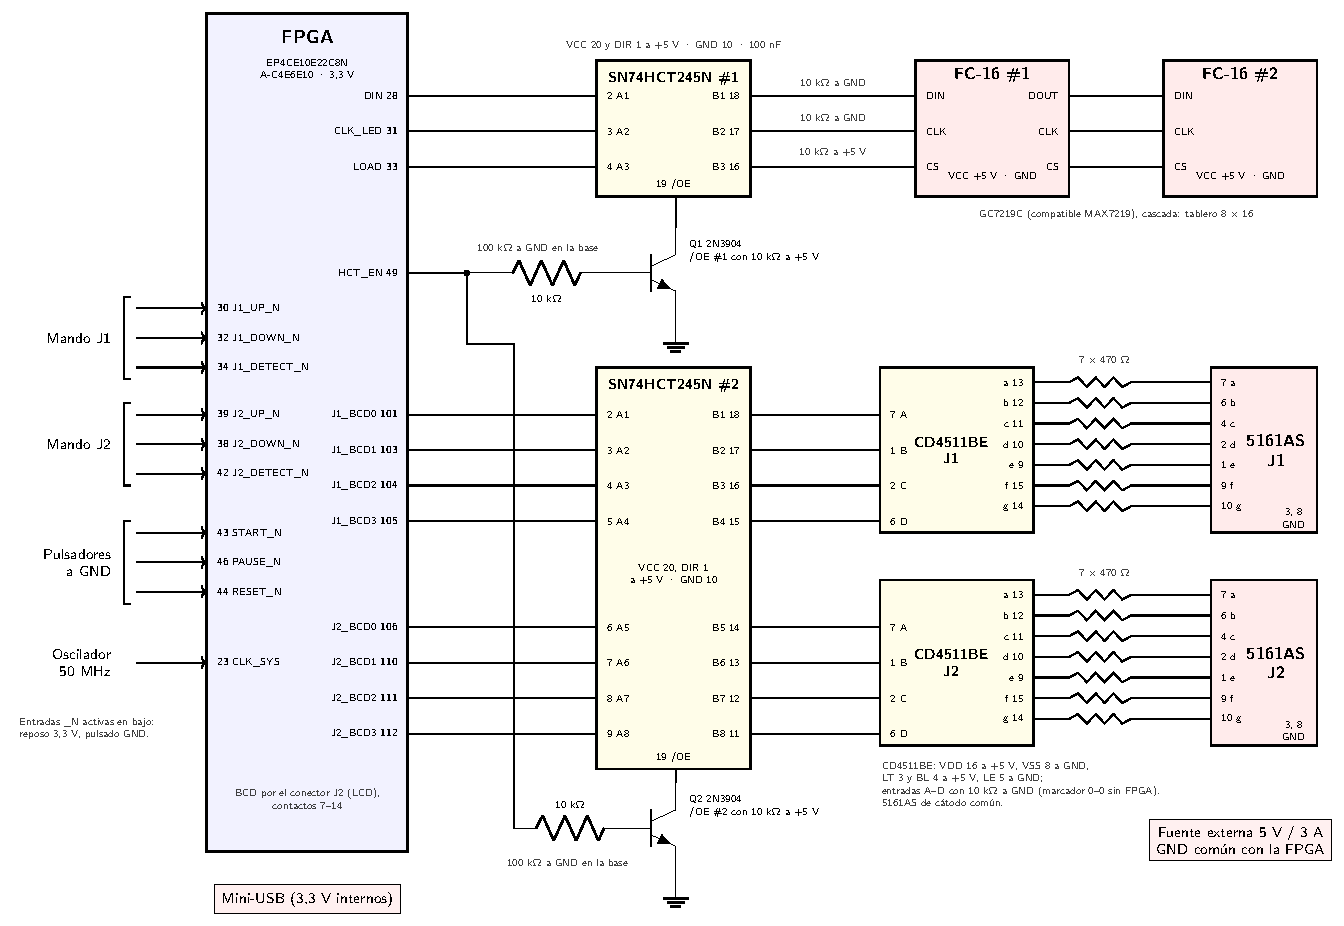
\includegraphics[width=0.94\textwidth]{fig_conexiones.pdf}
  \caption{Circuito de conexiones del prototipo, con los números de pin de la FPGA y de cada integrado. Los datos salen de las tablas de conexión de la memoria de F6.}
  \label{fig:conexiones}
\end{figure*}

\subsection{Listado de sensores y actuadores}

En este proyecto los ``sensores'' son las entradas con las que el jugador actúa sobre el juego, y los actuadores son los elementos que muestran el resultado. La Tabla~\ref{tab:sensores} los resume junto con los circuitos de interfaz que escogimos.

\begin{table}[!t]
\centering
\caption{Sensores, actuadores e interfaz escogidos}
\label{tab:sensores}
\footnotesize
\begin{tabularx}{\columnwidth}{@{}l c Y@{}}
\toprule
\textbf{Elemento} & \textbf{Cant.} & \textbf{Función} \\
\midrule
\multicolumn{3}{@{}l}{\textit{Entradas (sensores)}}\\
Mando cableado & 2 & UP y DOWN mueven la paleta; DETECT indica que el mando está conectado (pines 30, 32, 34 y 39, 38, 42) \\
Pulsador & 3 & START, PAUSE y RESET, activos en bajo (pines 43, 46, 44) \\
Oscilador de la tarjeta & 1 & Reloj de 50~MHz (pin 23) \\
\midrule
\multicolumn{3}{@{}l}{\textit{Actuadores}}\\
Módulo FC-16 $8\times8$ & 2 & Tablero de $8\times16$ LED; controlador GC7219C, compatible con MAX7219~\cite{max7219} \\
Display 5161AS & 2 & Un dígito de puntaje por jugador (cátodo común) \\
\midrule
\multicolumn{3}{@{}l}{\textit{Interfaz y alimentación}}\\
SN74HCT245N & 2 & Paso de 3,3~V a 5~V: \#1 matrices, \#2 marcador \\
CD4511BE & 2 & Decodificador BCD a siete segmentos \\
2N3904 & 2 & Habilitación del /OE de cada búfer \\
Resistencias & 31 & 14 de 470~Ω, 15 de 10~kΩ, 2 de 100~kΩ (y 2 condensadores de 100~nF) \\
Fuente de 5~V / 3~A & 1 & Matrices, búferes, decodificadores y displays \\
\bottomrule
\end{tabularx}
\end{table}

\subsection{Cambios frente a la propuesta}

Durante el desarrollo cambiamos algunas decisiones de la propuesta. Las dejamos explícitas porque afectan la evaluación del cumplimiento:

\begin{itemize}
\item \textbf{Controles.} La propuesta planteaba controles inalámbricos. En F5 los reemplazamos por mandos cableados: el diseño de F3 ya separaba la lógica del enlace en un módulo (\texttt{supervisor\_rf}) y la FSM ya tenía un estado de pérdida de enlace, así que reutilizamos esa estructura con la señal DETECT. Si un mando se desconecta, el juego pasa a PAUSA\_RF y solo continúa al reconectarlo y presionar START.
\item \textbf{Pelota.} En F0--F2 la pelota avanzaba en X cada 200~ms y en Y cada 400~ms. En F5 la cambiamos a movimiento diagonal, con X e Y en cada pulso, porque en la matriz real el juego se veía lento.
\item \textbf{Adaptador de niveles.} La propuesta mencionaba un SN74AHCT125~\cite{propuesta}; usamos dos SN74HCT245N porque necesitábamos once líneas y no solo tres.
\item \textbf{Orientación de la pantalla.} En F4 descubrimos que los módulos FC-16 tienen la columna~0 en el bit~0 y la fila~0 en el registro~8, al revés de lo que habíamos supuesto en F2. Corregimos dos módulos (\texttt{imagen} y \texttt{transmisor\_max7219}) y ajustamos los bancos de prueba.
\end{itemize}

% ============================================================================
% 4. Avance cuantitativo y cualitativo
% ============================================================================
\section{Avance respecto al cronograma}

\subsection{Avance cuantitativo}

La propuesta organizó el trabajo en diez actividades repartidas en cuatro semanas, S1 a S4~\cite{propuesta}. Para compararlas con lo hecho tomamos S1 como la semana del 26 de octubre al 1 de noviembre, de modo que este corte (15 de noviembre) cae al final de S3. La Fig.~\ref{fig:cronograma} pone lado a lado lo previsto y lo ejecutado, y la Tabla~\ref{tab:avance} da el porcentaje de cada actividad con su evidencia. Si se pesan igual las diez actividades, el avance global es de $875/10 \approx 88~\%$.

\begin{figure*}[!t]
  \centering
  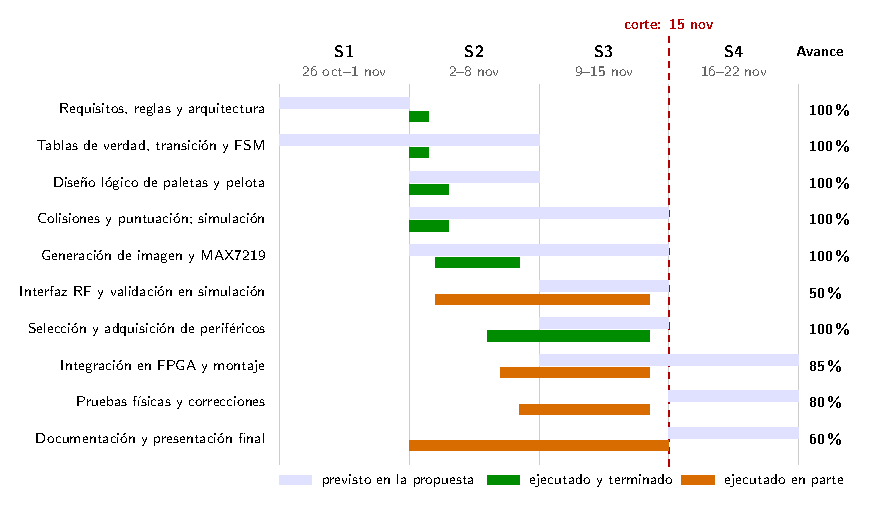
\includegraphics[width=0.82\textwidth]{fig_cronograma.pdf}
  \caption{Cronograma de la propuesta (barras claras) frente a lo ejecutado (barras oscuras). La línea punteada marca la fecha de este informe.}
  \label{fig:cronograma}
\end{figure*}

\begin{table*}[!t]
\centering
\caption{Avance de cada actividad del cronograma}
\label{tab:avance}
\footnotesize
\begin{tabularx}{\textwidth}{@{}l c c c Y@{}}
\toprule
\textbf{Actividad de la propuesta} & \textbf{Prevista} & \textbf{Ejecutada} & \textbf{Avance} & \textbf{Evidencia y observaciones} \\
\midrule
Requisitos, reglas y arquitectura & S1 & S2 & 100~\% & F0 rev.~1.2 (reglas, requisitos R01--R12) y F1 rev.~1.1 (contratos de 13 bloques) \\
Tablas de verdad, transición y FSM & S1--S2 & S2 & 100~\% & F2 rev.~1.2: tablas, ecuaciones, FSM del juego y del transmisor \\
Diseño lógico de paletas y pelota & S2 & S2 & 100~\% & F2 y módulos \texttt{paletas} y \texttt{pelota} de F3 \\
Colisiones y puntuación; simulación & S2--S3 & S2 & 100~\% & F3: 15 módulos, 19 bancos de prueba, 49/49 comprobaciones de integración \\
Generación de imagen y MAX7219 & S2--S3 & S2 & 100~\% & Simulación en F3 y prueba física en F4 (foto de las dos matrices) \\
Interfaz RF y validación en simulación & S3 & S2--S3 & 50~\% & La lógica de enlace se simuló (\texttt{tb\_supervisor\_rf}); no se compraron módulos RF y los mandos quedaron cableados \\
Selección y adquisición de periféricos & S3 & S2--S3 & 100~\% & Matrices, búferes, decodificadores, displays y fuente comprados y montados \\
Integración en FPGA y montaje & S3--S4 & S2--S3 & 85~\% & Montaje completo en protoboard (F6); faltan arranque autónomo y placas \\
Pruebas físicas y correcciones & S4 & S2--S3 & 80~\% & F4--F6: partida 9--6, victoria, RESET; faltan video y la revisión eléctrica de entradas \\
Documentación y presentación final & S4 & S2--S4 & 60~\% & Memorias F0--F7 y repositorio; faltan KiCad (F8), informe final y sustentación \\
\midrule
\multicolumn{3}{@{}l}{\textbf{Promedio de las diez actividades}} & \textbf{88~\%} & \\
\bottomrule
\end{tabularx}
\end{table*}

También medimos el avance con los doce requisitos de la especificación (Tabla~\ref{tab:requisitos}): nueve están cumplidos con evidencia de simulación y de hardware, y tres quedan parciales. Otros números que resumen el estado del diseño:

\begin{itemize}
\item \textbf{Simulación:} 19 de 19 bancos de prueba pasan, 14 de módulos y 5 de integración. Los de módulos recorren de forma exhaustiva las combinaciones de entrada que tienen sentido; por ejemplo, 87\,823 casos en colisiones, 65\,546 en la generación de imagen y 512 combinaciones en la FSM. Repetimos toda la batería con Icarus Verilog~\cite{icarus} y la dejamos corriendo automáticamente en el repositorio.
\item \textbf{Síntesis:} en F3 el núcleo ocupó 560 elementos lógicos y 276 registros, alrededor del 5~\% de los 10\,320 de la FPGA. La versión final (F6) compiló con 0 errores, 660 celdas lógicas, 22 pines de usuario y márgenes de $+6{,}686$~ns en \textit{setup} y $+0{,}186$~ns en \textit{hold} a 50~MHz.
\item \textbf{Hardware:} el juego completo funcionó en la tarjeta con las dos matrices, los dos mandos y el marcador al mismo tiempo.
\end{itemize}

\begin{table}[!t]
\centering
\caption{Estado de los requisitos de F0}
\label{tab:requisitos}
\footnotesize
\begin{tabularx}{\columnwidth}{@{}l Y l@{}}
\toprule
\textbf{Req.} & \textbf{Descripción corta} & \textbf{Estado} \\
\midrule
R01 & Controles independientes por jugador & \ok \\
R02 & Paletas dentro de las filas 0--6 & \ok \\
R03 & Avance de la pelota (cambiado a diagonal en F5) & \ok \\
R04 & Rebotes en paredes, paletas y esquinas & \ok \\
R05 & Cada gol suma una sola vez & \ok \\
R06 & Puntaje, RESET y victoria al llegar a 9 & \ok \\
R07 & Los 128 LED representan las posiciones & \ok \\
R08 & Inicialización y tramas de las dos matrices & \ok \\
R09 & Enlace RF, pérdida de enlace y recuperación & \parcial \\
R10 & Tensiones, corrientes y protección de GPIO & \parcial \\
R11 & PAUSE detiene y reanuda sin perder datos & \ok \\
R12 & Prioridades enlace $>$ PAUSE $>$ gol & \parcial \\
\bottomrule
\end{tabularx}
\end{table}

R09 y R12 quedan parciales porque se verificaron con la señal DETECT de los mandos cableados y no con un enlace inalámbrico real. R10 queda parcial porque medimos tensiones puntuales (5,22~V en la alimentación del búfer~\#2 y 3,27~V en HCT\_EN) pero no hicimos una revisión eléctrica completa, y Quartus mantiene una advertencia sobre las entradas de 3,3~V.

\subsection{Avance cualitativo}

Lo que más nos ayudó fue dedicar las dos primeras semanas a la especificación y al diseño formal, antes de escribir Verilog. Como las tablas de F2 ya estaban, la descripción en F3 fue casi directa y los bancos de prueba se pudieron escribir comparando contra esas mismas tablas. Por eso, cuando conectamos la primera matriz en F4, los errores que aparecieron no eran de lógica sino de orientación física de los módulos, y se corrigieron en dos archivos.

La integración por partes también funcionó: primero solo la pantalla (F4), luego los controles (F5) y por último el marcador (F6). En F6 probamos el marcador aislado, forzando valores BCD a mano, antes de conectarlo a la FPGA; eso nos dejó encontrar un problema con la habilitación del segundo búfer sin poner en riesgo la tarjeta. También tuvimos que liberar el pin~101 (que por defecto es nCEO) para usarlo como salida.

En cuanto a calendario, F0 a F5 terminaron antes de lo previsto, pero la interfaz inalámbrica no se hizo. Preferimos tener un juego completo y probado con mandos cableados a tener un enlace RF a medias, y dejamos la desviación documentada.

\begin{figure}[!t]
  \centering
  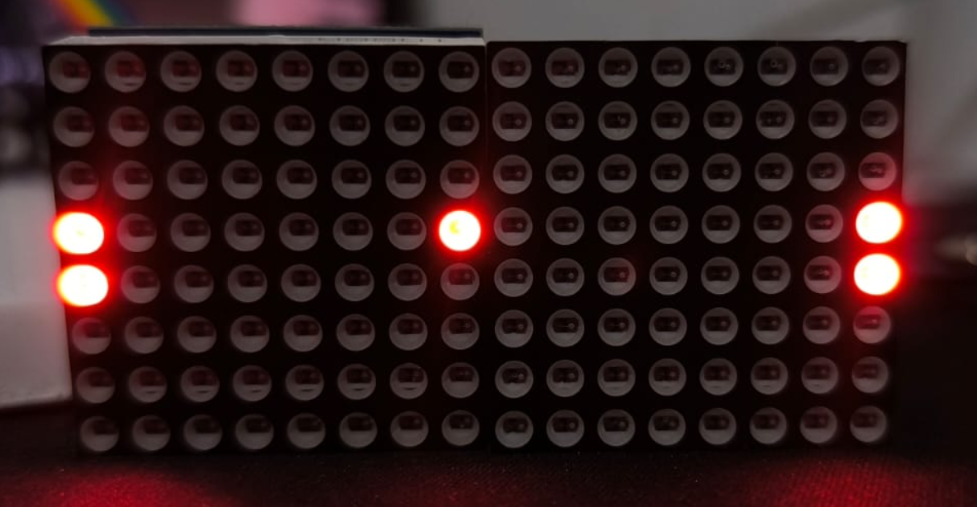
\includegraphics[width=\columnwidth]{F4_Prueba_Visual_MAX7219.png}
  \caption{Prueba de F4: las dos matrices en cascada muestran las paletas en los extremos y la pelota en su posición inicial.}
  \label{fig:f4}
\end{figure}

% ============================================================================
% 5. Desafíos para cerrar el proyecto
% ============================================================================
\section{Desafíos identificados para cerrar el proyecto}

\begin{enumerate}
\item \textbf{Controles inalámbricos.} Es el objetivo específico~5 de la propuesta. Tenemos que decidir con el profesor si se acepta el cambio a mandos cableados o si intentamos integrar módulos RF sencillos en lo que queda de tiempo. La arquitectura ya lo permite: bastaría con que los receptores entreguen UP, DOWN y una señal de enlace activa.
\item \textbf{Arranque autónomo.} Hoy la FPGA se programa por JTAG con un archivo \texttt{.sof}, que se borra al apagar. Para la presentación queremos grabar la memoria de configuración serial de la tarjeta (M25P16) con un archivo \texttt{.jic}, de modo que el juego arranque sin computador.
\item \textbf{Transitorios de encendido.} Con la fuente de 5~V encendida y la FPGA apagada o sin configurar, las matrices y los displays pueden mostrar patrones al azar. HCT\_EN depende del reloj de la FPGA y no detecta si los 5~V están presentes; falta estudiar una supervisión de alimentación o al menos fijar un procedimiento de encendido seguro.
\item \textbf{Revisión eléctrica de las entradas.} Quartus deja la advertencia 169177 sobre compatibilidad de las entradas LVTTL de 3,3~V. Debemos revisarla con la nota de aplicación AN~447~\cite{an447} y con la tensión de cada banco, para cerrar el requisito R10.
\item \textbf{Evidencia y pruebas de aceptación.} Las pruebas físicas de F5 y F6 se observaron pero no se grabaron. Antes de la sustentación hay que grabar video de una partida completa, tomar fotos del montaje y llenar la tabla requisito--prueba--evidencia.
\item \textbf{Repositorio al día.} Falta subir la memoria de F5 y el código final (\texttt{pong\_f5\_core}, \texttt{pong\_f6\_integracion\_top} y los módulos de los mandos cableados), y actualizar los bancos de prueba de la pelota al movimiento diagonal.
\item \textbf{Placas y presentación física (F8).} Queremos pasar el montaje de la protoboard a dos placas diseñadas en KiCad, una para mandos y pulsadores y otra para búferes, matrices y marcador.
\end{enumerate}

% ============================================================================
% 6. Bibliografía
% ============================================================================
\begin{thebibliography}{99}
\bibitem{propuesta} J. D. Ortiz Muñoz, D. E. Chivata Arias y D. F. Castro González, ``Diseño e implementación de un videojuego Pong mediante electrónica digital con FPGA y controles inalámbricos,'' propuesta corregida, Electrónica Digital~1, Univ. Nacional de Colombia, 2026.
\bibitem{guia} J. D. Ortiz Muñoz, D. E. Chivata Arias y D. F. Castro González, ``Guía metodológica de diseño, simulación y validación del videojuego Pong con FPGA,'' documento del proyecto, 2026.
\bibitem{f6} J. D. Ortiz Muñoz, D. E. Chivata Arias y D. F. Castro González, ``Fase 6: Integración, síntesis y montaje del videojuego Pong con marcadores externos de siete segmentos en FPGA,'' memoria técnica, rev.~1.0, 14 nov. 2026.
\bibitem{repo} Repositorio del proyecto ``pong-fpga-digital1'' (F0--F7, código, pruebas y hardware). [En línea]. Disponible: \url{https://github.com/dcastrogon-coder/pong-fpga-digital1}
\bibitem{mano} M. M. Mano y M. D. Ciletti, \textit{Digital Design}, 5.ª ed. Upper Saddle River, NJ, EE.~UU.: Pearson, 2013.
\bibitem{brown} S. Brown y Z. Vranesic, \textit{Fundamentals of Digital Logic with Verilog Design}, 3.ª ed. Nueva York, NY, EE.~UU.: McGraw-Hill, 2014.
\bibitem{tocci} R. J. Tocci, N. S. Widmer y G. L. Moss, \textit{Digital Systems: Principles and Applications}, 11.ª ed. Upper Saddle River, NJ, EE.~UU.: Pearson, 2011.
\bibitem{cyclone} Intel/Altera, \textit{Cyclone IV Device Handbook}, vol.~1, 2016.
\bibitem{an447} Intel/Altera, ``AN 447: Interfacing Cyclone III and Cyclone IV Devices with 3.3/3.0/2.5-V LVTTL/LVCMOS I/O Systems,'' nota de aplicación.
\bibitem{max7219} Analog Devices/Maxim Integrated, ``MAX7219/MAX7221: Serially interfaced, 8-digit LED display drivers,'' hoja de datos, rev.~6, 2021.
\bibitem{hct245} Texas Instruments, ``SN74HCT245: Octal bus transceivers with 3-state outputs,'' hoja de datos. [En línea]. Disponible: \url{https://www.ti.com/product/SN74HCT245}
\bibitem{cd4511} Texas Instruments, ``CD4511B CMOS BCD-to-7-segment latch decoder drivers,'' hoja de datos SCHS072B. [En línea]. Disponible: \url{https://www.ti.com/lit/ds/symlink/cd4511b.pdf}
\bibitem{disp} Shanghai Toplite Technology, ``TOP-CC-5161AS: Seven-segment display,'' hoja de datos, 2014.
\bibitem{icarus} S. Williams, ``Icarus Verilog.'' [En línea]. Disponible: \url{https://steveicarus.github.io/iverilog/}
\end{thebibliography}

\end{document}
